\section{Introduction}
\label{sec:introduction}

Cloud computing has revolutionized the way we store and process data, providing on-demand availability of computer system resources, especially data storage and computing power, without direct active management by the user. The term is generally used to describe data centers available to many users over the Internet. However, the current model of cloud computing is predominantly centralized, with a few major providers, such as Amazon Web Services (AWS), Google Cloud, and Microsoft Azure, dominating the market.

While these providers offer a wide range of services, from computation and storage to advanced analytics and machine learning tools, the centralized model is not without its issues and challenges. Users often find themselves locked into a single provider due to high switching costs, which can stifle competition and innovation. Centralized providers also present attractive targets for cyberattacks, and data breaches can lead to significant losses of sensitive data. Furthermore, the centralized model can lead to inefficiencies in resource allocation, as resources are often over-provisioned to handle peak demand.

\subsection{Background and Motivation}
\label{sec:background}

In response to these challenges, decentralized cloud computing has emerged as a promising alternative. This approach distributes data and processes across multiple machines, or nodes, each equipped with its own processing power and storage. This distribution can lead to more efficient resource allocation and utilization, as resources can be dynamically shared among nodes based on demand.

Our objective is to address the inherent issues of centralized cloud computing by constructing a secure and trustworthy system. This is achieved through the implementation of robust security measures and a reputation system, which collectively enhance the reliability and integrity of the platform.

Furthermore, we aim to promote transparency and democratic principles within the system by employing a decentralized matching engine and a Decentralized Autonomous Organization (DAO) model for governance. This approach is intended to stimulate competition and innovation in the field.

By lowering the barriers to becoming a cloud provider and offering a global rating system for all cloud providers, we enable developers to select providers based on their specific needs and preferences. This approach not only fosters a more competitive and innovative environment but also empowers developers by providing them with more choice and control over their cloud computing solutions.

\subsection{Academic research}

Some academic research was exploring the idea of decentralized cloud computing. For instance, Xu Chen's work on "Decentralized Computation Offloading Game for Mobile Cloud Computing" \cite{chen2014decentralized} proposes a game theoretic approach for achieving efficient computation offloading for mobile cloud computing. Another work by Sladana Jošilo and G. Dán titled "Selfish Decentralized Computation Offloading for Mobile Cloud Computing in Dense Wireless Networks" \cite{josilo2018selfish} also explores the concept of decentralized computation offloading.

Kunal et al.~\cite{kunal2019overview} discuss the potential of fog computing, an intermediate layer between users and the cloud server, to reduce latency and improve service delivery.
Similarly, Nguyen et al.~\cite{nguyen2020integration} present a comprehensive review of the integration of blockchain and Cloud of Things, highlighting the potential of this approach to address challenges in decentralization, data privacy, and network security.

More recently, Wenjuan Li et al. proposed a blockchain-based trust management system in cloud computing \cite{li2021blockchain}.
Chegini et al.~\cite{chegini2021process} propose the automation of tasks, methods, and processes in the IoT-Fog-Cloud ecosystem to deal with big data and heterogeneity challenges. Finally, Espinel Sarmiento et al.~\cite{sarmiento2021decentralized} survey the field of Software Defined Networks (SDN) applied to distributed Cloud-Edge infrastructures' management.


\subsection{Industry projects}

In recent years, several industry projects have attempted to build decentralized cloud platforms. These platforms leverage blockchain technology to create a network of independent node providers that can store data or run arbitrary workloads in a decentralized fashion, and highly resilient to malicious actors.

\begin{itemize}
    \item Filecoin (\url{https://filecoin.io/}): Filecoin is a decentralized storage system that aims to "store humanity's most important information". It is an open-source project that builds a decentralized network for storing and retrieving files, incentivized through the Filecoin cryptocurrency. However, while Filecoin does provide a marketplace for unused storage, it does not focus on compute resources. Our proposed platform, on the other hand, is more comprehensive and includes both storage and compute resources.

    \item Storj (\url{https://www.storj.io/}): Storj is a decentralized cloud storage platform that uses blockchain technology and cryptography to secure online files. Instead of maintaining data in a centralized server, Storj breaks it into smaller pieces, encrypts it, and distributes it across its network. However, similarly to Filecoin, Storj does not provide a marketplace for compute resources. Our platform aims to provide a marketplace for both storage and compute resources.

    \item Sia (\url{https://sia.tech/}): Sia is a decentralized storage platform secured by blockchain technology. The Sia Storage Platform leverages underutilized hard drive capacity worldwide to create a data storage marketplace that is more reliable and lower cost than traditional cloud storage providers. Similarly to Filecoin and Storj, Sia does not offer compute resources or a reputation-based system for node providers. Our platform includes these features.

    \item Golem (\url{https://golem.network/}): Golem is a global, open-source, decentralized supercomputer that anyone can access. It's made up of the combined power of user machines, from PCs to entire data centers. Golem is a decentralized supercomputer, which is similar to our proposal. However, Golem is more focused on providing a platform for compute-intensive tasks rather than a general-purpose cloud platform. Our platform aims to be more versatile, accommodating a wider range of workloads.

    \item iExec (\url{https://iex.ec/}): iExec is a decentralized marketplace for cloud computing resources. It allows decentralized applications (DApps) running on blockchain to access the computing resources they need. Applications running on iExec still need to run through the Consensus protocol, which slows down execution. Therefore, iExec is primarily focused on serving decentralized applications (DApps) running on the blockchain. Our platform aims to serve a broader range of applications, not just DApps.

    \item Arweave (\url{https://www.arweave.org/}): Arweave is a new type of storage that backs data with sustainable and perpetual endowments, allowing users and developers to store data permanently. Arweave does not provide compute resources or a marketplace for them. Our platform aims to provide both.

    \item DFINITY (\url{https://dfinity.org/}): DFINITY's Internet Computer is a decentralized cloud computing platform that aims to host both backend and frontend stack, which in turn allows developers to host their entire applications completely on the Internet Computer. This makes Internet Computer similar to our proposal. However, applications on the Internet Computer still need to run through the Consensus protocol, which significantly limits their speed. Our platform aims to provide a more general-purpose cloud platform, accommodating a wider range of workloads, and offer significantly higher performance.
\end{itemize}

These works highlight the growing interest in decentralized cloud computing and the potential benefits it can offer.
However, despite these efforts there is still a need for a comprehensive solution that addresses the issues of the current cloud computing paradigm while leveraging the benefits of decentralization. This is the problem that our proposed decentralized cloud platform aims to solve and in the following sections we provide an outline of how we plan to do this.

\begin{figure*}[ht]
    \centering
    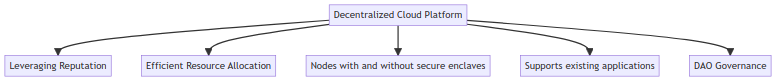
\includegraphics[width=\textwidth]{figures/proposed-solution.png}
    \caption{An illustration of the proposed solution.}
\end{figure*}
